%!TEX root = /Users/laura/Repositories/HandwritingRecognition/report/main.tex
\IEEEPARstart{N}{ational} archives often contain invaluable documents for researchers in different fields, e.g. historians or language researches. Currently most of these records are effectively useless, not only are these fragile documents hard to access, reading them is difficult. This makes any attempt at an analysis of their contents time intensive. Digitalizing these texts as images makes them more accessible, but any extensive analysis of their contents is still tedious. For computational analysis of the contents of these texts we need the textual information they contain in a machine readable format. The process that transforms these images of handwritten text into a machine readable format is called offline handwriting recognition \cite{graves2009offline}.

This variant of handwriting recognition is in general considered to be more difficult than its counterpart, online handwriting recognition. As the last not only uses the resulting image but also the trajectory of the pen as the image is drawn. The focus of this paper is on offline handwriting recognition of roman scripts. In \cref{ss:introduction:offlineHWR} the different stages in a bottom-up offline handwriting recognition system are shortly discussed and some of the techniques used for these steps are introduced. The method that is subject of this paper is introduced in \cref{ss:introduction:theMethod}.

\subsection{Offline Handwriting Recognition}
\label{ss:introduction:offlineHWR}
	Broadly speaking one can distinguish two different offline systems: top-down and bottom-up. The first performs recognition by direct comparison to a lexicon of descriptions \cite{impedovo2012fundamentals}. Systems in the second category start by classifying strokes, or characters, and then work their way up to the whole text. As our proposed recognizer is bottom-up the rest of this section will focus on this approach. Bottom-up recognizers have five major stages: 
	\begin{enumerate*}[label=(\roman*)]
		\item \label{it:introduction:preprocessing} preprocessing,
		\item \label{it:introduction:segmentation} segmentation,
		\item \label{it:introduction:representation} representation,
		\item \label{it:introduction:trainingRecognition} recognition and
		\item \label{it:introduction:postProcessing} post processing
	\end{enumerate*}
	\cite{arica2001overview}. \Crefrange{sss:introduction:offline:preprocessing}{sss:introduction:offline:postprocessing} shortly discuss \crefrange{it:introduction:preprocessing}{it:introduction:postProcessing}, respectively. 

	\subsubsection{Preprocessing}
	\label{sss:introduction:offline:preprocessing}
		The goal of preprocessing is to produce a ```clean' document in the sense that a sufficient amount of shape information, high compression and low noise on a normalized image is obtained"\cite[p. 219]{arica2001overview}. This is done by reducing the noise in the image, normalizing the data and compressing the amount of information that has to be retained. It should be noted that anyone of these steps can be skipped, depending on the images.

	\subsubsection{Segmentation}
	\label{sss:introduction:offline:segmentation}
		This stage aims to segment the `clean' document into its subcomponents. This stage consists of two steps: external segmentation and internal segmentation. The first step, external segmentation, is the isolation of the various components that make up a text, i.e paragraphs, sentences and words. Internal segmentation is concerned with the separation of letters within a word. Three different approaches to character segmentation have been developed \cite{casey1996survey}: explicit segmentation, implicit segmentation and mixed strategies. The first dissects the image into smaller images with meaningful components. Implicit segmentation is based on recognition, given a set of classes the image is searched for components that match. Mixed strategies combine the explicit and implicit approaches by over segmenting the input image with an explicit approach and then searching for the optimal segmentation using the implicit approach. 

		An example of the last method is over segmentation. This method fragments words into primitives that are either characters or part of characters. The optimal segmentation of a word is found by validation, i.e. testing a set of segmentation hypotheses that are generated by merging neighboring primitives and invoking a classifier to score the combination. The best scoring combination of primitives is selected as the final segmentation \cite{camastra2007svm}. One disadvantage of this approach is its computational complexity.	An over segmented word with $n$ possible character boundaries can be segmented in \bigOh{2^{n}} ways, each of these has to be tested, which is computationally expensive. To reduce this complexity one can test for characters from left to right, and accept a sub image as a character if it is recognized as such by some validation measure. This reduces the number of combinations to test. A disadvantage of this approach is its sensitivity to chain failure, i.e. failures of the segmentation algorithm on earlier characters negatively influence the performance on later characters. The risk of chain failure can be reduced by selecting an optimal, according to some criterion, segmentation point at each step\cite{lee2012binary}.

	\subsubsection{Representation}
	\label{sss:introduction:offline:representation}
		\Cref{it:introduction:representation} transforms the images of characters into some representation that is accepted by the classifier. Although it is possible to use the images, most recognition system use some feature vector to represent the image. 

		A relatively simple representation is the crossings feature vector. This vector contains the number of crossings for each row and column in the scaled image. A crossing if a transition from foreground to background, or from background to foreground \cite{HWR:features1,HWR:features2}.

	\subsubsection{Recognition}
	\label{sss:introduction:offline:recognition}
		\Cref{it:introduction:trainingRecognition} applies pattern recognition to handwriting recognition. Some classifier is used to assign a predefined class, one of the possible characters, to some unknown sample, the representation of a character. 

		One of the more simple classifiers is the \Knn classifier. This system assigns the most frequent class of its \knnk neighbors to a previously unseen pattern. The \knnk neighbors are determined via some distance measure. It has been shown that this relatively simple classifier works well for the recognition of handwritten characters when the Euclidean distance measure is used\cite{lee1991handwritten,smith1994handwritten,ha1997off}. One of the disadvantages of \knn is its computational and spatial complexity. The computational complexity can be reduced by using a k-dimensionality (k-d) tree, if the number of training patterns is smaller than the dimensionality of a feature vector \cite{bhatia2010survey}.

	\subsubsection{Post-Processing}
	\label{sss:introduction:offline:postprocessing}
		The last step, post processing, uses context information to improve the results of the previous stage. A simple post processing step would be to compute the distance between the read word and all words in the lexicon and assume that the word in the lexicon with the smallest distance to the read word is the written word. 

	\begin{figure}[t]
		\centering
		\subfloat[]{
			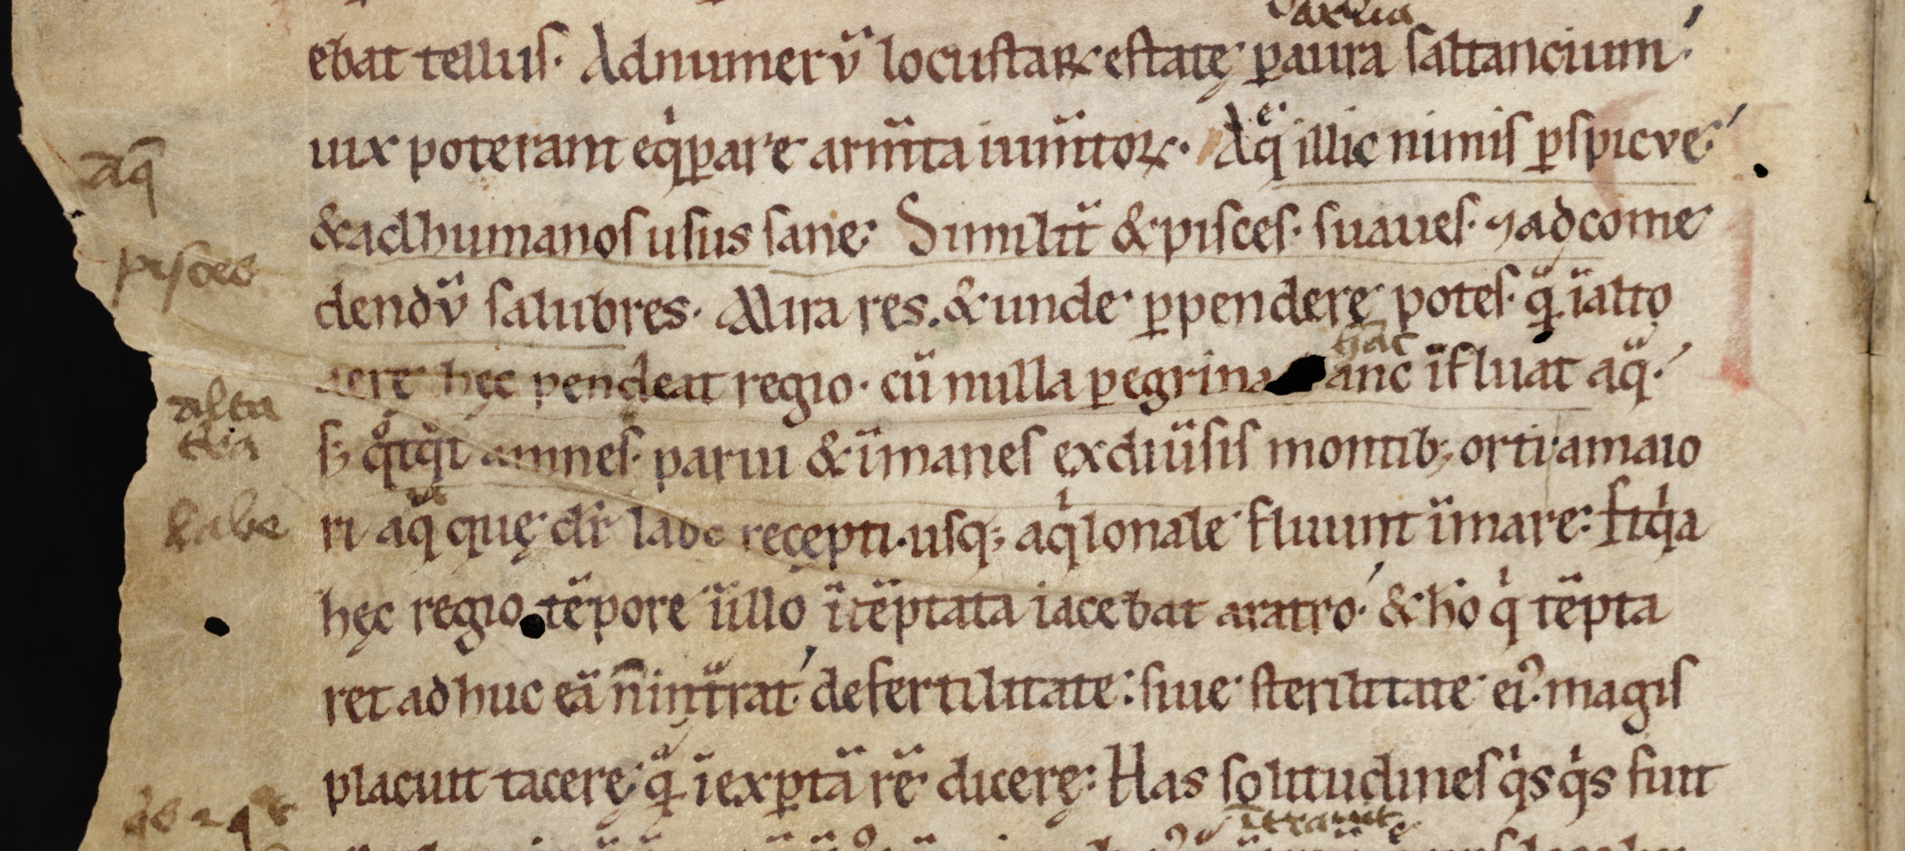
\includegraphics[width=0.6\columnwidth, height=0.1\textheight, keepaspectratio]{individual/img/introduction/bohemians.png}%
			\label{fig:introduction:bohemians}%
		}
		\hfil
		\subfloat[]{
			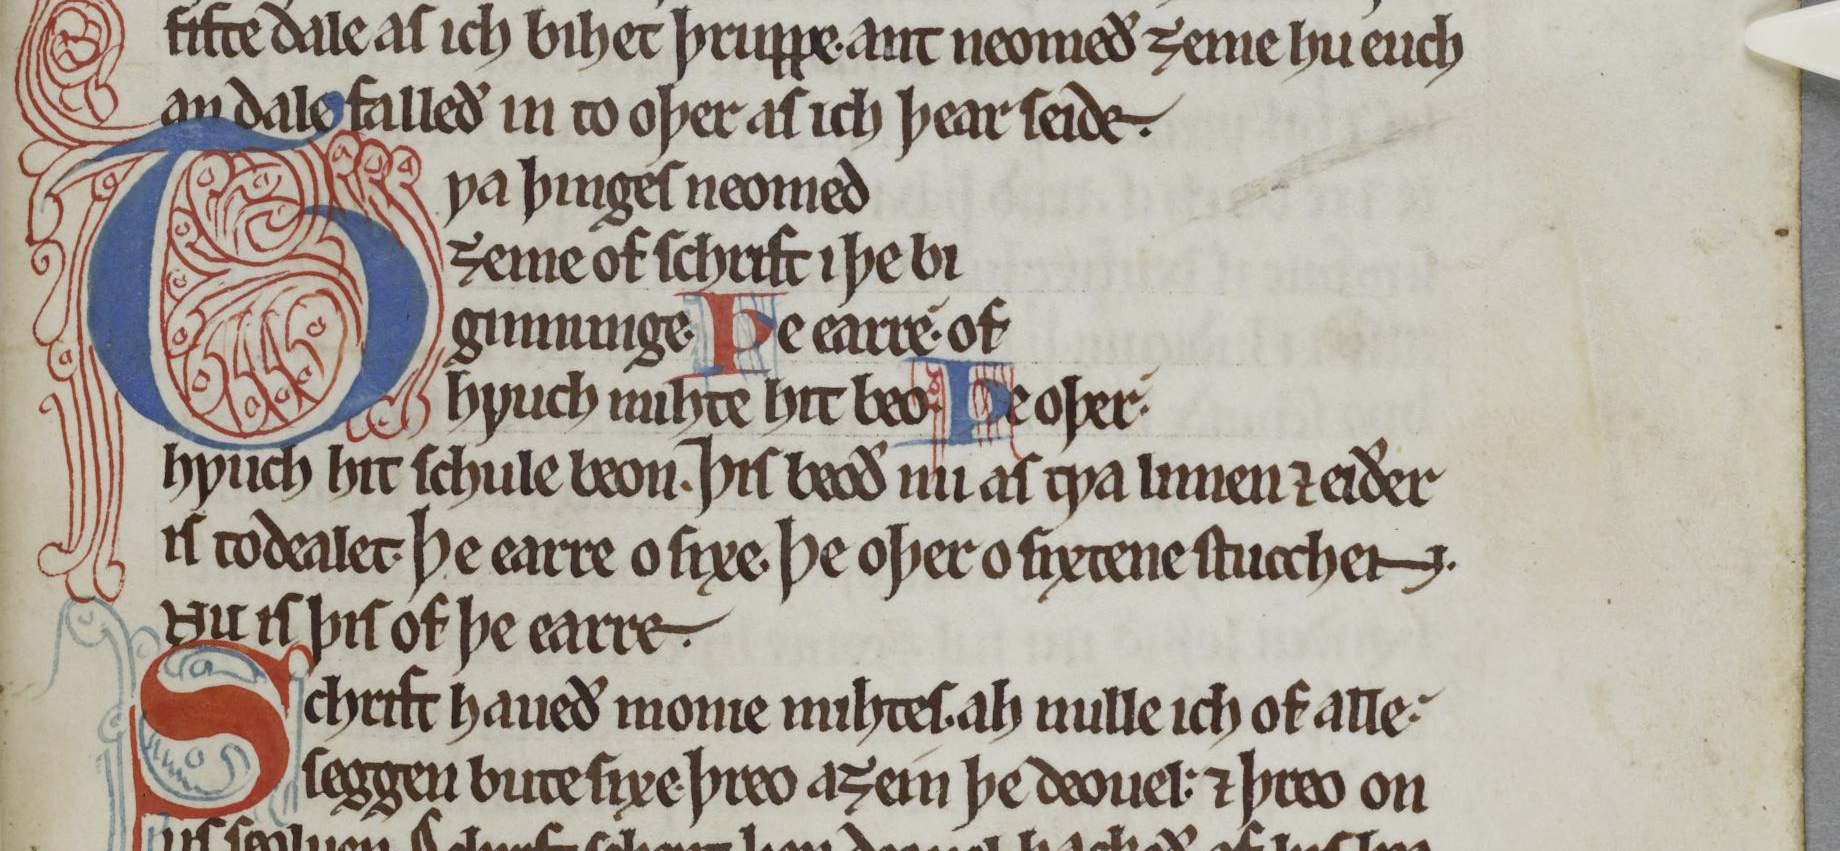
\includegraphics[width=0.6\columnwidth, height=0.1\textheight, keepaspectratio]{individual/img/introduction/oldEnglishHomilies.png}%
			\label{fig:introduction:oldEnglishHomilies}%
		}
		\caption{Part of a page from \protect\subref{fig:introduction:bohemians} ``Chronicle of the Bohemians" and \protect\subref{fig:introduction:oldEnglishHomilies} ``Old English Homilies". Word bounding boxes are shown as opaque blue rectangles, character bounding boxes as red rectangles.}
		\label{fig:introduction:exampleData}
	\end{figure}

\begin{figure}[b]
	\centering
	\subfloat[]{
		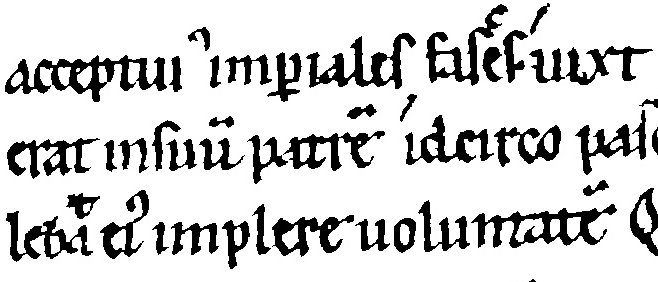
\includegraphics[width=0.45\columnwidth]{shared/img/after_lum.png}%
		\label{fig:methods:preprocessing:lumNormalization:after}%
	}	
	\hfill
	\subfloat[]{
		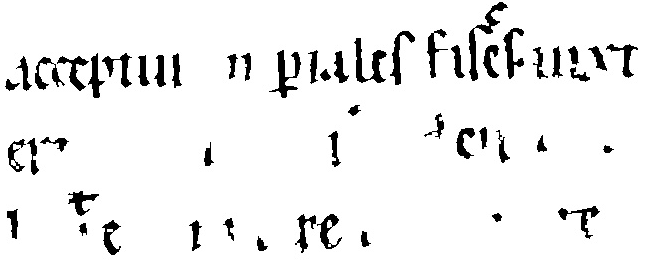
\includegraphics[width=0.45\columnwidth]{shared/img/before_lum.png}%
		\label{fig:methods:preprocessing:lumNormalization:before}%
	}
	\caption{A thresholded image with \protect\subref{fig:methods:preprocessing:lumNormalization:after} and without \protect\subref{fig:methods:preprocessing:lumNormalization:before} luminosity normalization.}
	\label{fig:methods:preprocessing:lumNormalization}
\end{figure}

\subsection{The Proposed Recognizer}
\label{ss:introduction:theMethod}
	Our system aims to transcribe the text of two twelfth century manuscripts, ``Chronicle of the Bohemians", which is written in Latin, and ``Old English Homilies" which is in English and Latin \cite{OldEnglishHomilies}. \Cref{fig:introduction:exampleData} shows a part of one page from these two texts.

	\Cref{s:methods} discusses how our recognizer works, its results are presented and discussed in \cref{s:results} and \ref{s:discussion}, respectively. \Cref{s:conclusion} concludes the paper.